\newpage

En el ejercicio dos se introdujeron dos familias nuevas: \textbf{Random} y \textbf{Gimnasios por grupo} que fueron explicadas apropiadamente. Como la idea es estudiar en promedio que sucede con las distancias al crecer la cantidad de elementos total del mapa (pokeparadas + gimnasios), las experimentaciones de este test se centrarán en tratar de mejorar esas distancias mediante las heurísticas introducidas en este punto ($2-opt$ y $Swap$).\\\\

Para realizar los tests se tomaron dos rangos de tamaños: 5 a 20 elementos (pokeparadas + gimnasios) y 70 a 470 en saltos de 50 elementos.
Para el primer rango se tomó el total del tamaño como cantidad de instancias aleatorias por cada tamaño y para el segundo rango se tomó un 10\% del total de elementos como cantidad de instancias aleatorias.
Se realizan las busquedas locales promediando los tiempos y distancias para todas las instancias de cada tamaño. Y se obtienen los porcentajes de mejora relativos a cada tamaño con respecto al promedio de las distancias del algoritmo goloso. 

\subsubsection*{Random}


\\\\

\begin{figure}[h] 
 \centering
  \subfloat[Distancias]{
    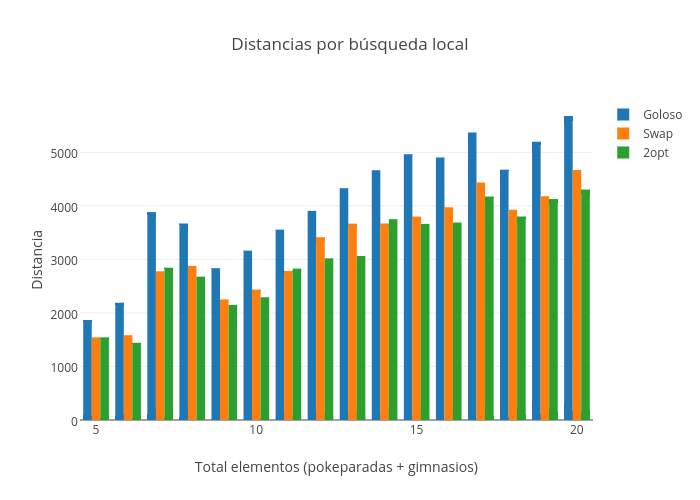
\includegraphics[width=0.45\textwidth]{./EJ3/distanciasLocales20.png}}
       \label{fig:randomDist1}
  \subfloat[Porcentaje de mejora]{
    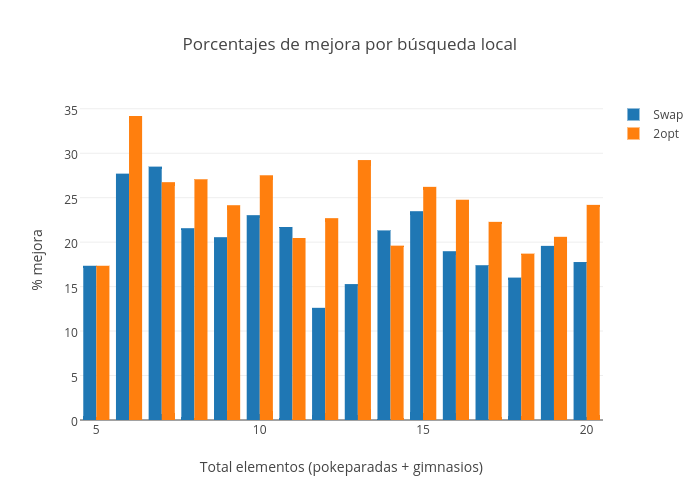
\includegraphics[width=0.45\textwidth]{./EJ3/mejoraLocales20.png}}
    \label{fig:randomMejora1}
\end{figure}

   \vspace*{0.3cm} \vspace*{0.3cm}
  \begin{center}
	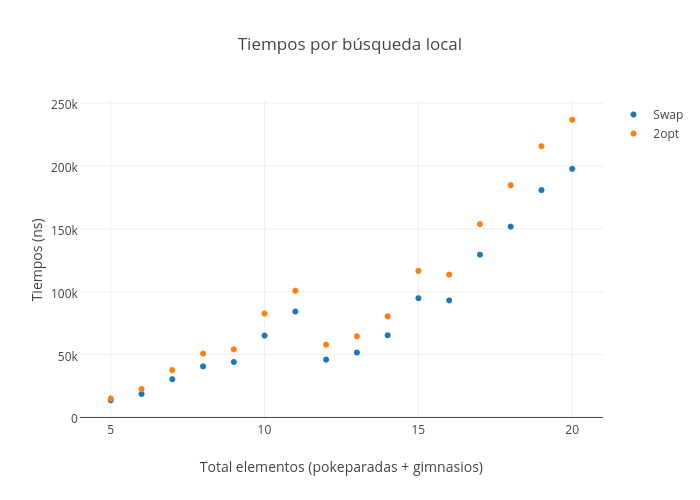
\includegraphics[scale=0.40]{./EJ3/tiemposLocales20.png}
	\label{fig:randomTiempos1}	
	\\{\textit{Tiempos}}
  \end{center}
  \vspace*{0.3cm} 

Como puede observarse...asdasdasdasdasdasdasdasdasdadadadasdaddasddaadasdasdasdadasdasdasd
adassdasdasdasdasdasdasdasdasdasasdadaddasd
adasdasdsd
\\\\
\begin{figure}[h] 
 \centering
  \subfloat[Distancias]{
    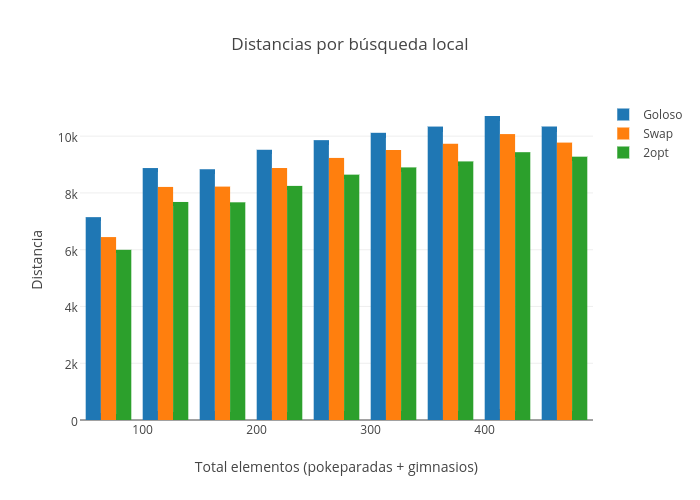
\includegraphics[width=0.45\textwidth]{./EJ3/distanciasLocales470.png}}
       \label{fig:randomDist2}
  \subfloat[Porcentaje de mejora]{
    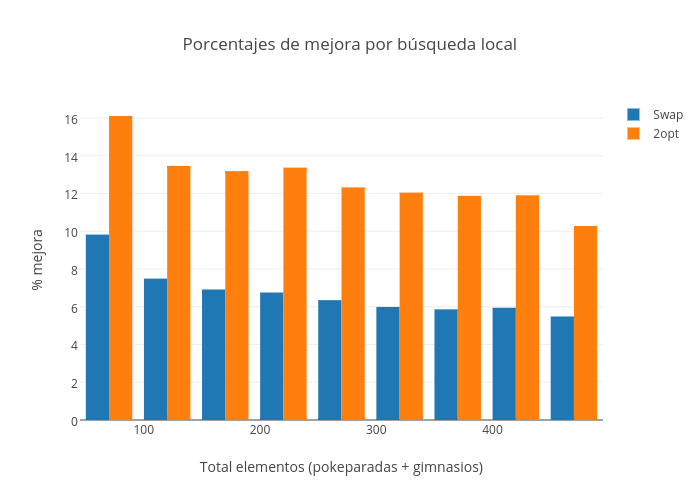
\includegraphics[width=0.45\textwidth]{./EJ3/mejoraLocales470.png}}
    \label{fig:randomMejora2}
    \end{figure}
 
   \vspace*{0.3cm} \vspace*{0.3cm}
  \begin{center}
	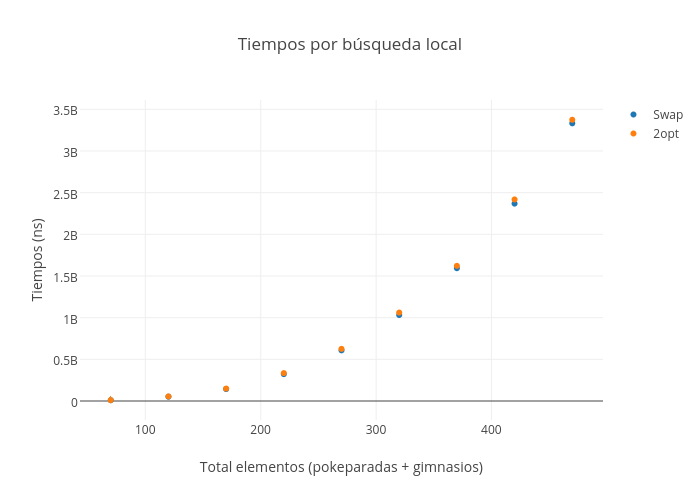
\includegraphics[scale=0.40]{./EJ3/tiemposLocales470.png}
	\label{fig:randomTiempos2}	
	\\{\textit{Tiempos}}
  \end{center}
  \vspace*{0.3cm} 

Como puede observarse...asdasdasdasdasdasdasdasdasdadadadasdaddasddaadasdasdasdadasdasdasd
adassdasdasdasdasdasdasdasdasdasasdadaddasd
adasdasdsd  
\\\\
 
\newpage
\subsubsection*{Gimnasios por grupos}

Como puede observarse...asdasdasdasdasdasdasdasdasdadadadasdaddasddaadasdasdasdadasdasdasd
adassdasdasdasdasdasdasdasdasdasasdadaddasd
adasdasdsd
\\\\

\begin{figure}[h] 
 \centering
  \subfloat[Distancias]{
    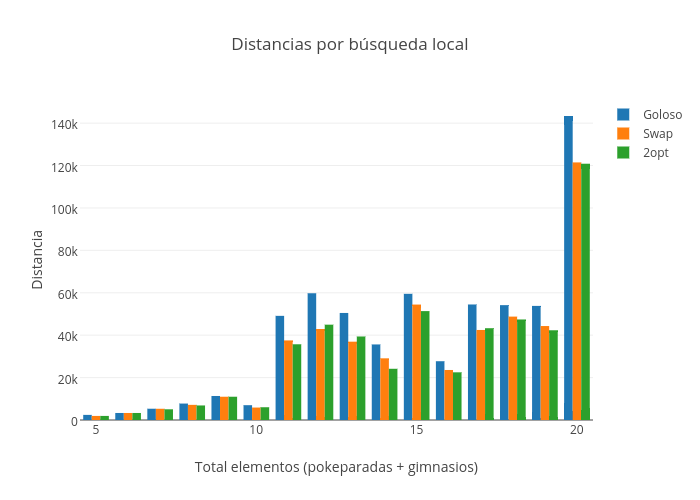
\includegraphics[width=0.45\textwidth]{./EJ3/distanciasLocales20cuad.png}}
       \label{fig:gruposDist1}
  \subfloat[Porcentaje de mejora]{
    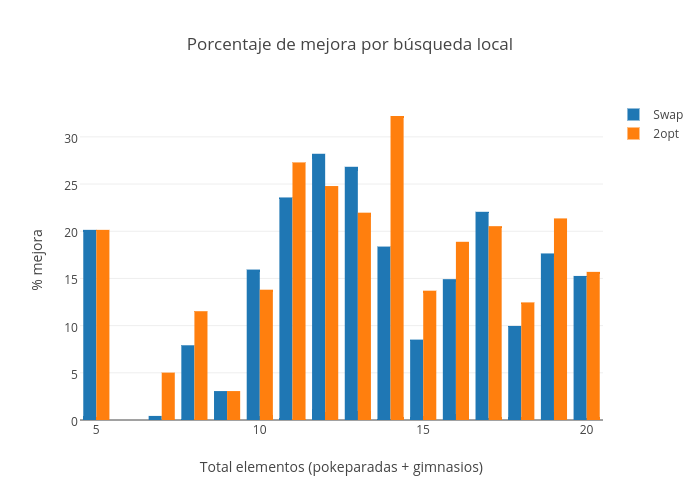
\includegraphics[width=0.45\textwidth]{./EJ3/mejoraLocales20cuad.png}}
    \label{fig:gruposMejora1}
    \end{figure}
 
   \vspace*{0.3cm} \vspace*{0.3cm}
  \begin{center}
	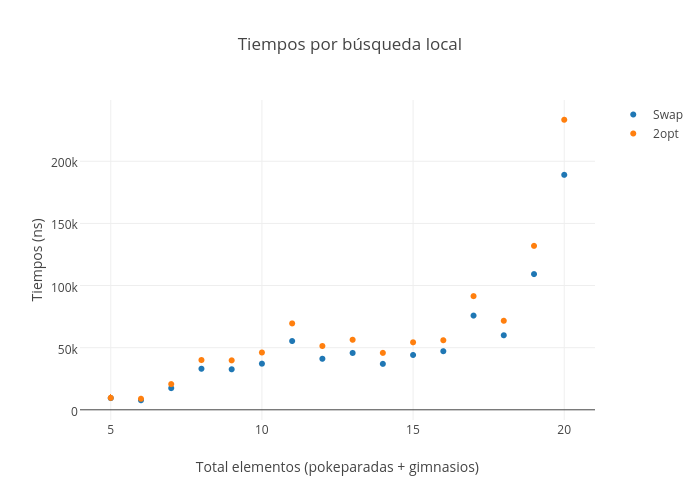
\includegraphics[scale=0.40]{./EJ3/tiemposLocales20cuad.png}
	\label{fig:gruposTiempos1}	
	\\{\textit{Tiempos}}
  \end{center}
  \vspace*{0.3cm} 

Como puede observarse...asdasdasdasdasdasdasdasdasdadadadasdaddasddaadasdasdasdadasdasdasd
adassdasdasdasdasdasdasdasdasdasasdadaddasd
adasdasdsd
\\\\

\begin{figure}[h] 
 \centering
  \subfloat[Distancias]{
    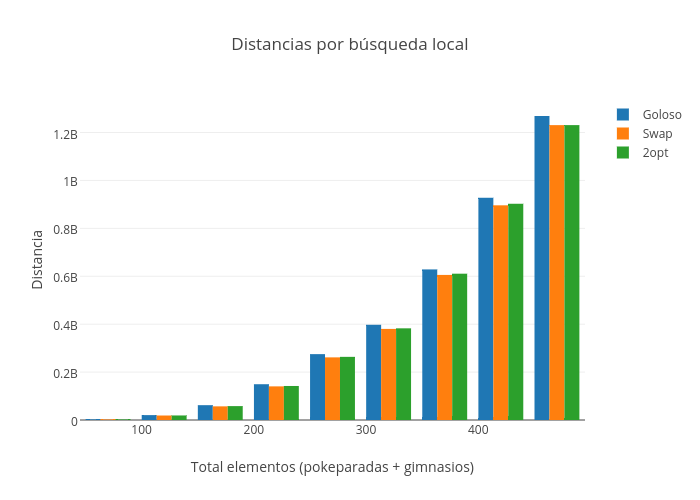
\includegraphics[width=0.45\textwidth]{./EJ3/distanciasLocales470cuad.png}}
       \label{fig:gruposDist2}
  \subfloat[Porcentaje de mejora]{
    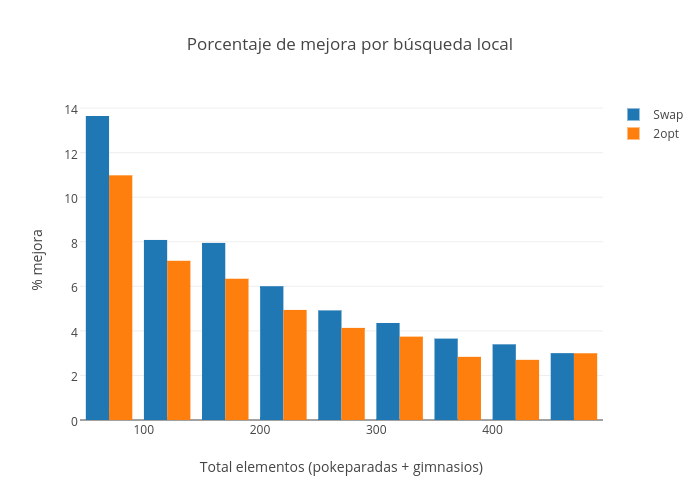
\includegraphics[width=0.45\textwidth]{./EJ3/mejoraLocales470cuad.png}}
    \label{fig:gruposMejora2}
    \end{figure}
 
   \vspace*{0.3cm} \vspace*{0.3cm}
  \begin{center}
	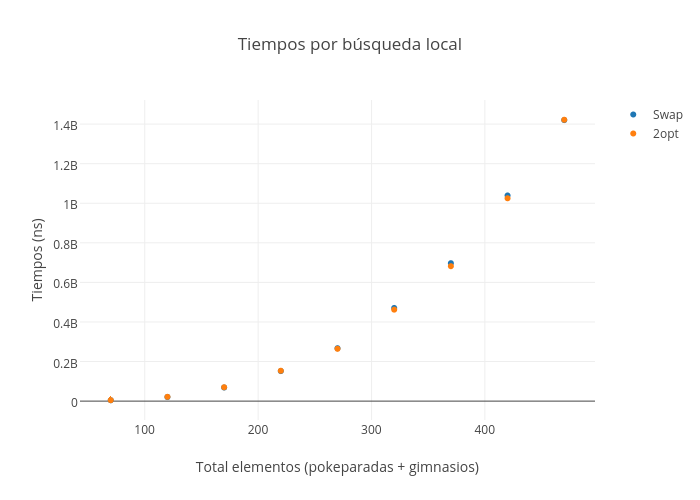
\includegraphics[scale=0.40]{./EJ3/tiemposLocales470cuad.png}
	\label{fig:gruposTiempos2}	
	\\{\textit{Tiempos}}
  \end{center}
  \vspace*{0.3cm} 
 
Como puede observarse...asdasdasdasdasdasdasdasdasdadadadasdaddasddaadasdasdasdadasdasdasd
adassdasdasdasdasdasdasdasdasdasasdadaddasd
adasdasdsd
\\\\
  